\section{Seleção dos Modelos de Aprendizado de Máquina}
\label{cap:7.3}

Como já vimos, a estrutura de particionamento de blocos do formato AV1 é composta por uma árvore que pode atingir até o sexto nível de profundidade. O particionamento de algum nível de profundidade em quatro novos ramos pode ser feito somente nos cinco primeiros níveis, conforme discutido no capítulo \ref{cap:5}. Naquele capítulo, inclusive, abordamos a distribuição da aplicação do particionamento para cada nível de profundidade e, como pudemos constatar, o software de referência do codificador AV1 opta pela divisão em quatro novos blocos de tamanho 8$\times$8 em apenas 16\% das vezes em que está processando a profundidade 3. Como visto no capítulo \ref{cap:5}, a opção por blocos iguais ou inferiores a 8$\times$8, em vídeos HD1080, se aproxima de no máximo 5\% no vídeo. Inclusive, a desativação nativa da profundidade 5 em vídeos de resolução UHD faz com que esse percentual de área dedicada a blocos pequenos seja significativamente menor. Desta forma, o ganho de tempo em se acelerar a escolha de subparticionamento rápido em blocos 8$\times$8 e 16$\times$16 é mínimo. Assim, na proposta de transcodificador rápido desenvolvido neste capítulo, não iremos utilizar modelos preditivos para as profundidades 3 e 4. Todavia, há outros três níveis de particionamento cuja aceleração com uso de modelos de aprendizado de máquina pode ser vantajosa, sendo eles de 128$\times$128 para 64$\times$64, de 64$\times$64 para 32$\times$32 e de 32$\times$32 para 16$\times$16.

Em vista desse fato, combinando o número de níveis de quantização utilizados utilizados nos experimentos apresentados nesta tese (quatro valores, como apresentamos no capítulo \ref{cap:4}) mais as três profundidades consideradas para decisão de particionamento, obtém-se um total de 12 conjuntos de amostras para treinamento, conforme listados abaixo:

\begin{itemize}
    \item Conjunto 1: CQ 20, particionamento de 128$\times$128 em 64$\times$64;

    \item Conjunto 2: CQ 20, particionamento de 64$\times$64 em 32$\times$32;

    \item Conjunto 3: CQ 20, particionamento de 32$\times$32 em 16$\times$16;

    \item Conjunto 4: CQ 32, particionamento de 128$\times$128 em 64$\times$64;

    \item Conjunto 5: CQ 32, particionamento de 64$\times$64 em 32$\times$32;

    \item Conjunto 6: CQ 32, particionamento de 32$\times$32 em 16$\times$16;

    \item Conjunto 7: CQ 43, particionamento de 128$\times$128 em 64$\times$64;

    \item Conjunto 8: CQ 43, particionamento de 64$\times$64 em 32$\times$32;

    \item Conjunto 9: CQ 43, particionamento de 32$\times$32 em 16$\times$16;

    \item Conjunto 10: CQ 55, particionamento de 128$\times$128 em 64$\times$64;

    \item Conjunto 11: CQ 55, particionamento de 64$\times$64 em 32$\times$32;

    \item Conjunto 12: CQ 55, particionamento de 32$\times$32 em 16$\times$16;
\end{itemize}

Com o objetivo de simplificar o balanceamento dos dados brutos a fim de permitir uma automatização mais direta das fases de treinamento e teste dos modelos, como apresentamos na subseção \ref{cap:7.2.2}, optamos por um balanceamento de 50\%-50\%, ou seja, cada rótulo dos dados de treinamento e de teste é representado a mesma quantidade de vezes no conjunto de amostras. Algum balanceamento dos dados se faz necessário, pois como visto no capítulo \ref{cap:5}, só no CQ 55, o primeiro nível de profundidade tende a se subparticionar em 99,42\% das vezes. Logo, havendo 99,42\% das amostras com rótulos positivo (isto é, particionar) e 0,58\% das amostras com rótulo negativo (isto é, não particionar), justifica-se a aplicação de algum balanceamento de dados, principalmente considerando que há 12 conjuntos diferentes de dados de treinamento.

\citet{bib:livroimbalanced} apresenta várias técnicas de balanceamento de dados e qualquer uma delas irá incluir algum tipo de viés nos dados, nos quais dois são os principais: \textit{oversampling} e \textit{undersampling}. Segundo o autor, a técnica de \textit{oversampling} pode aumentar a probabilidade de gerar um modelo preditivo com sobreajuste dos dados, uma vez que faz cópias das amostras da classe minoritária para se equivaler em número aos da classe majoritária. Desta forma, um modelo sobreajustado pode apresentar resultados estatísticos que são aparentemente precisos, mas na verdade só respondem bem a casos conhecidos e não são bons em predizer casos inéditos. Por outro lado, a técnica de \textit{undersampling} descarta uma quantidade significativa de amostras, e isso é problemático, pois a perda de tais amostras pode dificultar o aprendizado do modelo para casos que estejam no limite de decisão entre as instâncias minoritária e majoritária, resultando em uma perda no desempenho da classificação. Considerando essas observações de \citet{bib:livroimbalanced} mais a desproporção dos desbalanceamentos observados, ponderamos que adaptar 0,58\% dos dados para se equivaler a 99,42\% dos demais rótulos não é eficiente. Assim, optamos por utilizar a técnica de balanceamento de dados com \textit{undersampling} aleatório.

É possível obter uma relação da quantidade máximas e teóricas dos dados de treinamento, a despeito do seu desbalanceamento, pois esses valores são diretamente proporcionais à quantidade de vídeos utilizados, de sua resolução e da quantidade de quadros utilizados na codificação. Dessa forma, considerando os vídeos de treinamento expostos na seção \ref{cap:7.1}, a quantidade máxima de amostras para cada rótulo que podemos obter para cada profundidade é de 47.040 (para profundidade 0), 194.880 (profundidade 1) e 817.740 (profundidade 2). No entanto, essas amostras estão desbalanceadas. Portanto, após realizar o processo de balanceamento exposto no parágrafo anterior, obtemos o número de amostras para cada rótulo apresentadas nas Tabelas \ref{tab:XIX}, \ref{tab:XX}, \ref{tab:XXI}, \ref{tab:XXII} e \ref{tab:XXIII} para as transcodificações VP8-AV1, VP9-AV1, H.264/AVC-AV1, H.265/HEVC-AV1 e H.266/VVC-AV1, respectivamente. Nessas tabelas, também são apresentadas a quantidade de amostras para os conjuntos de testes.

\begin{table}
\begin{center}
\caption{Quantidade de amostras de treinamento e teste de modelos preditivos para a transcodificação VP8-AV1 após o balanceamento.}
\label{tab:XIX}
\footnotesize

\begin{tblr}{
    colspec = {l|l|r|r|r},
    hlines,
    row{even} = {gray9},
    cell{5}{1} = {gray9},
    cell{9}{1} = {gray9}
}
\hline
\SetCell[c=2]{c} && \SetCell[c=3]{c}\textbf{Profundidade}    \\
\textbf{CQ}                  & \textbf{Conjunto de} & \textbf{0 (128$\times$128)} & \textbf{1 (64$\times$64)} & \textbf{2 (32$\times$32)} \\
\SetCell[r=2]{c}20 & treinamento & 29.485      & 115.893   & 238.375   \\
                   & teste       & 29.487      & 114.063   & 188.627   \\
\SetCell[r=2]{c}32 & treinamento & 35.385      & 119.601   & 229.431   \\
                   & teste       & 31.595      & 101.505   & 164.651   \\
\SetCell[r=2]{c}43 & treinamento & 36.951      & 109.673   & 183.869   \\
                   & teste       & 31.741      & 78.815    & 121.035   \\
\SetCell[r=2]{c}55 & treinamento & 37.093      & 91.247    & 123.445   \\
                   & teste       & 31.913      & 65.897    & 68.029   \\

\hline
\end{tblr}
\end{center}
\end{table}

\begin{table}
\begin{center}
\caption{Quantidade de amostras de treinamento e teste de modelos preditivos para a transcodificação VP9-AV1 após o balanceamento.}
\label{tab:XX}
\footnotesize

\begin{tblr}{
    colspec = {l|l|r|r|r},
    hlines,
    row{even} = {gray9},
    cell{5}{1} = {gray9},
    cell{9}{1} = {gray9}
}
\hline
\SetCell[c=2]{c} && \SetCell[c=3]{c}\textbf{Profundidade}    \\
\textbf{CQ}                  & \textbf{Conjunto de} & \textbf{0 (128$\times$128)} & \textbf{1 (64$\times$64)} & \textbf{2 (32$\times$32)} \\
\SetCell[r=2]{c}20 & treinamento & 38.537 & 133.935 & 251.863   \\
                   & teste       & 30.941 & 89.017 & 145.783   \\
\SetCell[r=2]{c}32 & treinamento & 42.191 & 132.475 & 232.079   \\
                   & teste       & 37.055 & 87.115 & 171.525   \\
\SetCell[r=2]{c}43 & treinamento & 42.293 & 125.575 & 184.545   \\
                   & teste       & 37.201 & 758.95 & 121.567   \\
\SetCell[r=2]{c}55 & treinamento & 42.443 & 107.471 & 120.343   \\
                   & teste       & 37.337 & 66.111 & 62.661   \\

\hline
\end{tblr}
\end{center}
\end{table}

\begin{table}
\begin{center}
\caption{Quantidade de amostras de treinamento e teste de modelos preditivos para a transcodificação H.264/AVC-AV1 após o balanceamento.}
\label{tab:XXI}
\footnotesize

\begin{tblr}{
    colspec = {l|l|r|r|r},
    hlines,
    row{even} = {gray9},
    cell{5}{1} = {gray9},
    cell{9}{1} = {gray9}
}
\hline
\SetCell[c=2]{c} && \SetCell[c=3]{c}\textbf{Profundidade}    \\
\textbf{CQ}                  & \textbf{Conjunto de} & \textbf{0 (128$\times$128)} & \textbf{1 (64$\times$64)} & \textbf{2 (32$\times$32)} \\
\SetCell[r=2]{c}20 & treinamento & 30.233 & 113.225 & 226.393   \\
                   & teste       & 32.107 & 120.487 & 190.105   \\
\SetCell[r=2]{c}32 & treinamento & 35.949 & 112.485 & 215.039   \\
                   & teste       & 36.943 & 110.657 & 171.583   \\
\SetCell[r=2]{c}43 & treinamento & 37.015 & 103.269 & 172.291   \\
                   & teste       & 37.157 & 78.757 & 118.595   \\
\SetCell[r=2]{c}55 & treinamento & 37.127 & 91.473 & 112.135   \\
                   & teste       & 37.321 & 65.807 & 56.141   \\

\hline
\end{tblr}
\end{center}
\end{table}

\begin{table}
\begin{center}
\caption{Quantidade de amostras de treinamento e teste de modelos preditivos para a transcodificação H.265/HEVC-AV1 após o balanceamento.}
\label{tab:XXII}
\footnotesize

\begin{tblr}{
    colspec = {l|l|r|r|r},
    hlines,
    row{even} = {gray9},
    cell{5}{1} = {gray9},
    cell{9}{1} = {gray9}
}
\hline
\SetCell[c=2]{c} && \SetCell[c=3]{c}\textbf{Profundidade}    \\
\textbf{CQ}                  & \textbf{Conjunto de} & \textbf{0 (128$\times$128)} & \textbf{1 (64$\times$64)} & \textbf{2 (32$\times$32)} \\
\SetCell[r=2]{c}20 & treinamento & 34.025 & 114.627 & 232.023   \\
                   & teste       & 21.287 & 60.171 & 125.563   \\
\SetCell[r=2]{c}32 & treinamento & 28.883 & 86.755 & 163.465   \\
                   & teste       & 20.879 & 47.105 & 111.405   \\
\SetCell[r=2]{c}43 & treinamento & 27.771 & 81.985 & 137.667   \\
                   & teste       & 31.823 & 73.165 & 126.757   \\
\SetCell[r=2]{c}55 & treinamento & 21.307 & 62.815 & 80.835   \\
                   & teste       & 15.893 & 46.909 & 40.937   \\

\hline
\end{tblr}
\end{center}
\end{table}

\begin{table}
\begin{center}
\caption{Quantidade de amostras de treinamento e teste de modelos preditivos para a transcodificação H.266/VVC-AV1 após o balanceamento.}
\label{tab:XXIII}
\footnotesize

\begin{tblr}{
    colspec = {l|l|r|r|r},
    hlines,
    row{even} = {gray9},
    cell{5}{1} = {gray9},
    cell{9}{1} = {gray9}
}
\hline
\SetCell[c=2]{c} && \SetCell[c=3]{c}\textbf{Profundidade}    \\
\textbf{CQ}                  & \textbf{Conjunto de} & \textbf{0 (128$\times$128)} & \textbf{1 (64$\times$64)} & \textbf{2 (32$\times$32)} \\
\SetCell[r=2]{c}20 & treinamento & 35.405 & 125.719 & 147.691\\
                   & teste       & 36.579 & 123.265 & 86.685\\
\SetCell[r=2]{c}32 & treinamento & 36.935 & 116.395 & 206.447\\
                   & teste       & 37.031 & 97.013 & 141.231\\
\SetCell[r=2]{c}43 & treinamento & 36.981 & 106.637 & 172.987\\
                   & teste       & 37.181 & 78.023 & 102.277\\
\SetCell[r=2]{c}55 & treinamento & 37.099 & 95.047 & 112.299\\
                   & teste       & 37.313 & 68.183 & 54.689\\

\hline
\end{tblr}
\end{center}
\end{table}


Na subseção \ref{cap:7.1.3}, citamos que são considerados 9.526.572 combinações candidatas de hiperparâmetros para o algoritmo de aprendizado de máquina CART \cite{bib:livroCART}. É necessário selecionar o melhor candidato dentre todos, a fim de submeter esse candidato à Fase 4 do \textit{pipeline}. A forma mais justa de descobrir qual deles apresenta o melhor resultado de \textit{F1-Score} é realizar o treinamento completo com todos os candidatos e obter a média estatística de cada um desses modelos, após a rodada de testes. No entanto, a aplicação da técnica de busca exaustiva para encontrar o melhor modelo não é viável em termos de tempo de processamento. Apesar de cada combinação de hiperparâmetros apresentar um tempo de treinamento relativamente fixo de apenas seis segundos para o conjunto com maiores amostras (profundidade 2 e CQ 20, conforme Tabela \ref{tab:XX}), ao considerarmos o universo completo de combinações (de 9.526.572), o treinamento em busca exaustiva para todos os 12 modelos seria finalizado em 21,8 anos.

Desse modo, é fundamental que se aplique alguma metodologia de treinamento rápido a fim de providenciar um candidato vencedor em tempo hábil. Há diversas formas discutidas na literatura para lidar com esse problema, cada uma com suas características positivas e negativas, sendo que a resolução desse problema, inclusive, é uma área de forte interesse na academia. Uma das técnicas mais conhecidas envolve a busca por grade \cite{bib:randomsearch} (do inglês, \textit{Grid Search}), onde devem ser definidos os valores de cada hiperparâmetro que se deseja testar e, em seguida, todas as combinações possíveis desses valores serão testadas. No entanto, essa técnica é muito custosa, caso existam muitos valores a serem testados. Por outro lado, principalmente visando acelerar a busca por hiperparâmetros, também pode ser encontrada na literatura a técnica de busca por grade aleatória (do inglês, \textit{Random Grid Search}, RGS). Nesta técnica, os valores a serem testados para cada hiperparâmetro são definidos pelo par de limites: inferior e superior. Desta forma, valores aleatórios dentro desse intervalo-limite são testados e avaliados, podendo-se dar maior exploração de busca em sub-intervalos cujos resultados sejam mais apurados.

Contudo, apesar da técnica RGS ser mais eficiente em termos de uso de recursos computacionais do que a técnica de busca por grade simples, uma série de candidatos não são testados, o que pode ocasionar em encontrar combinações que sejam categorizados como máximos locais. Ou seja, existe uma possibilidade de não serem encontrados os máximos globais. Dessa forma, optamos por utilizar outra técnica de avaliação de hiperparâmetros que permite avaliar todas as suas combinações, tornando possível aproximar o resultado de máximos globais e, ainda assim, ter um tempo de processamento rápido: a busca por hiperparâmetros com validação cruzada e com cortes randomizados e recursivos \cite{bib:halvingrandomsearch}, do inglês, \textit{Halving Random Search with Cross Validation} (HRSCV).

A Figura \ref{fig:29} exemplifica o funcionamento da HRSCV, na qual cada ciclo corresponde a três fases de processamento: seleção, treinamento/teste e avaliação. No entanto, em vez de processar treinamentos com o conjunto completo de amostras, como ocorre com a busca exaustiva ou a RGS, a HRSCV seleciona aleatoriamente uma parte das amostras e realiza o treinamento de todas as combinações de hiperparâmetros por meio de uma validação cruzada com cinco subconjuntos mutuamente exclusivos. A etapa de seleção de amostras é importante, pois, a cada novo ciclo, a HRSCV seleciona mais amostras disponíveis no conjunto, a um crescimento definido por $fator$. Essa variável, $fator$, é determinante para definir o crescimento do custo computacional empregado na HRSCV. Iniciando com um conjunto de tamanho definido pelo usuário (preferencialmente múltiplo de cinco), cada nova iteração da HRSCV aumenta o tamanho da amostra em $fator$ vezes, ao mesmo tempo que o número de combinações de hiperparâmetros decai em $fator$ vezes. Portanto, apesar de tecnicamente o produto entre combinações de hiperparâmetros e o tamanho da amostra de treinamento ser o mesmo ao longo dos ciclos, o custo computacional de treinar um modelo com cada vez mais amostras é maior. Dessa forma, a HRSCV garante um treinamento significativamente rápido no primeiro ciclo, mesmo considerando um conjunto grande de combinações de hiperparâmetros, por dispor de um número ínfimo de amostras. A cada novo ciclo, aumentamos o custo computacional para treinamento e, ao mesmo tempo, ganhamos maior confiança nos resultados obtidos com os testes. Por essa razão, o custo computacional da HRSCV é diretamente proporcional aos valores definidos (tamanho da amostra inicial, $fator$ e número de combinações de hiperparâmetros), podendo apresentar custos superiores ao de uma técnica de busca exaustiva, caso os valores definidos não forem ajustados de acordo com as necessidades.

\begin{figure}
    \centering
    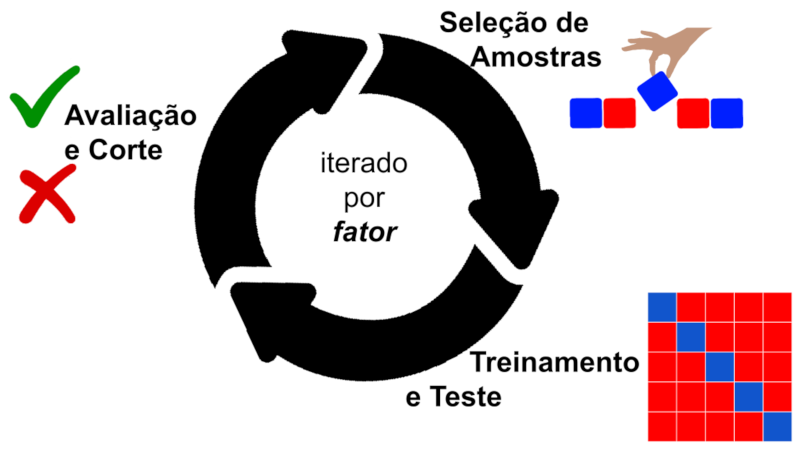
\includegraphics[width=0.5\textwidth]{FIGURES/fig_29.png}
    \caption{Fluxo geral de execução da técnica de avaliação de hiperparâmetros \textit{Halving Random Search with Cross Validation}. Fonte: Elaborada pelo autor.}
    \label{fig:29}
\end{figure}

Uma das formas que a HRSCV possui para limitar o seu custo computacional é definir as condições de parada de sua execução, sendo elas: (a) não haver mais combinações de hiperparâmetros a serem comparados e (b) não haver mais amostras suficientes para iniciar um novo ciclo. A primeira condição, basicamente, indica que foi encontrado o melhor modelo dentro de todas as combinações de hiperparâmetros. Já a segunda condição sinaliza que não há um conjunto de amostras com o tamanho necessário para iniciar o ciclo, sendo finalizada a HRSCV contendo não o vencedor, mas uma lista de N melhores combinações de hiperparâmetros até o momento, em ordem decrescente de pontuação. Conforme já definimos anteriormente, as propostas deste capítulo utilizam como métrica para esta pontuação o valor de \textit{F1-Score}.

Expostas essas informações, é possível estimar quantos ciclos de execução são executados, com base nos valores iniciais da técnica HRSCV, cujos valores de combinações e amostras são, respectivamente, calculados pelas equações \ref{eq:9} e \ref{eq:10}. O tamanho de combinações de hiperparâmetros inicial já é conhecido (9.526.572) e o valor de $fator$ deve ser adequado ao problema, mas obrigatoriamente maior que 1. Vamos manter o tamanho de $fator$ padrão, que é de 2, ou seja, a cada ciclo, o número de combinações cai pela metade enquanto o tamanho da amostra dobra. Por fim, devemos definir a quantidade de amostras que são utilizadas no primeiro ciclo da HRSCV. Em sua documentação em \citet{bib:halvingrandomsearch}, o recomendado é que este valor seja no mínimo cinco vezes $fator$ amostras por número de atributos usados para treinar o modelo. Como veremos na seção \ref{cap:7.4}, são utilizados 25 atributos para treinamento dos modelos; logo, o recomendado é utilizar ao menos 250 amostras no primeiro ciclo.

\begin{equation}
    \label{eq:9}
    Amostras_{ciclo}=Amostras_{inicial}*fator^{ciclo - 1}
\end{equation}

\begin{equation}
    \label{eq:10}
    Combinacoes_{ciclo}=Combinacoes_{inicial}*fator^{ciclo - 1}
\end{equation}

Conhecendo as condições de início da HRSCV aplicadas para geração dos modelos propostos, é possível estimar quantos ciclos seriam executados para cada um dos subconjuntos de treinamento, conforme explicitados na Tabela \ref{tab:XXIV}. Nesta tabela, apresentamos todos os ciclos possíveis até atingir a condição de parada (a), ou seja, de encontrar a melhor combinação de hiperparâmetros. Todavia, não temos um conjunto de treinamento que contenha dois bilhões de amostras, como exigiria o 24$^\circ$ ciclo apresentado na Tabela \ref{tab:XXIV}. Ainda assim, evidenciamos que o menor conjunto de treinamento (profundidade 0 para o CQ 55, conforme Tabela \ref{tab:XXII}), pode ser processado em oito ciclos, retornando uma lista com mais de 37 mil combinações de hiperparâmetros. Já o maior conjunto de treinamento (da profundidade 2 para o CQ 20), pode ser processado em 11 ciclos, retornando uma lista com 9 mil combinações de hiperparâmetros.

\begin{table}
\begin{center}
\caption{Número de candidatos e amostras necessárias para execução de cada ciclo da técnica HRSCV, conforme condições definidas nesta tese.}
\label{tab:XXIV}
\footnotesize

\begin{tblr}{
    colspec = {l|r|r},
    hlines,
    row{even} = {gray9}
}
\hline

\textbf{Ciclo} & \textbf{Candidatos} & \textbf{Amostras}      \\
1     & 9.526.572  & 250           \\
2     & 4.763.286  & 500           \\
3     & 2.381.643  & 1.000         \\
4     & 1.190.822  & 2.000         \\
5     & 595.411    & 4.000         \\
6     & 297.705    & 8.000         \\
7     & 148.853    & 16.000        \\
8     & 74.426     & 32.000        \\
9     & 37.213     & 64.000        \\
10    & 18.607     & 128.000       \\
11    & 9.303      & 256.000       \\
12    & 4.652      & 512.000       \\
13    & 2.326      & 1.024.000     \\
14    & 1.163      & 2.048.000     \\
15    & 581        & 4.096.000     \\
16    & 291        & 8.192.000     \\
17    & 145        & 16.384.000    \\
18    & 73         & 32.768.000    \\
19    & 36         & 65.536.000    \\
20    & 18         & 131.072.000   \\
21    & 9          & 262.144.000   \\
22    & 5          & 524.288.000   \\
23    & 2          & 1.048.576.000 \\
24    & 1          & 2.097.152.000 \\
\hline
\end{tblr}
\end{center}
\end{table}


De cada uma dessas 12 listas retornadas ao fim da execução da HRSCV, capturamos os 20 melhores, unificando-os para obter uma lista de até 240 combinações de hiperparâmetros. há a possibilidade de existirem combinações repetidas nas listas, logo, as repetições são eliminadas. Só então, aplicamos o treinamento e o teste completo para os modelos, de forma a gerar uma lista com dados estatísticos de todos esses candidatos. Com esses processos de filtragem, reduzimos o tempo de processamento de 21 anos de uma busca exaustiva para menos de 10 horas.

Em posse da lista dos 240 candidatos e dos seus valores estatísticos, removemos todos os que não atingem ao menos 0,75 pontos de AUC, mesmo que para apenas um único modelo. Como a AUC informa a probabilidade de o modelo retornar uma resposta positiva corretamente, determinamos que o mínimo valor aceitável seja de 0,75, por ser a metade entre o pior (0,5) e o melhor (1,0) AUC possível. Após essa filtragem final, calculamos a média do \textit{F1-Score} de todos os modelos que foram treinados sob uma mesma combinação de hiperparâmetros, ordenando-os por valor de \textit{F1-Score} médio. Aquele candidato que estiver em primeiro lugar nesta lista, será utilizado na Fase 4 do \textit{pipeline}, a fim de ser aplicado na aceleração da transcodificação.
